


\chapter{Runway Usage}\label{app:RWY_usage}


\begin{figure}[h]
    \centering
    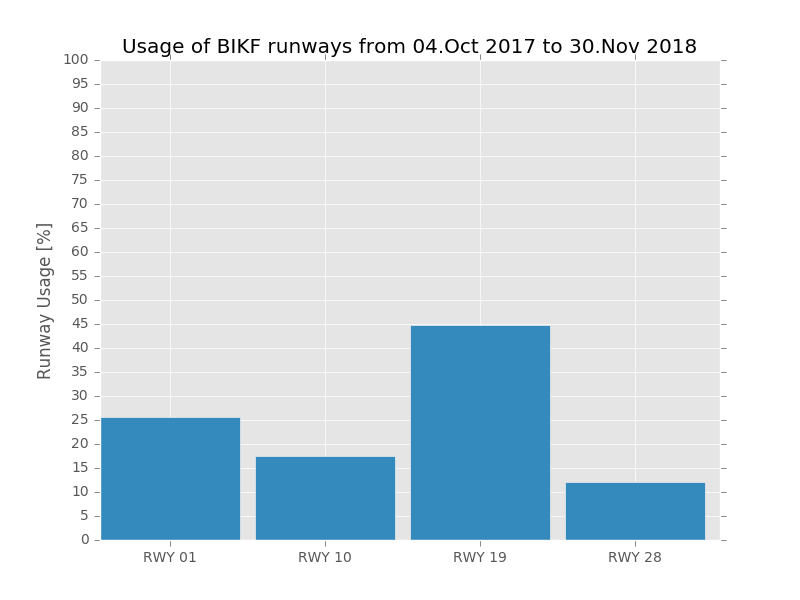
\includegraphics[width=0.8\textwidth]{graphics/fig_runway_usage_2017-10-04_to_2018-11-30.png}
    \caption[Runway usage at BIKF]{Overall runway usage at BIKF for a period of one year since October 2017. Almost half of all arrivals during that period (44,7\%) use RWY-19, followed by RWY-01 (25,7\%) and RWY-10 (17.6\%). The summer traffic favoured RWY-19 with 52.8\%~(Figure~\ref{fig:runway_usage_summer}), while during the winter season some of those arrivals were diverted towards RWY-01 and RWY-10~(Figure~\ref{fig:runway_usage_summer}). RWY-28 was least used despite its rapid-exit TWY B-1.}
    \label{fig:runway_usage}
\end{figure}

\begin{figure}[h]
    \centering
    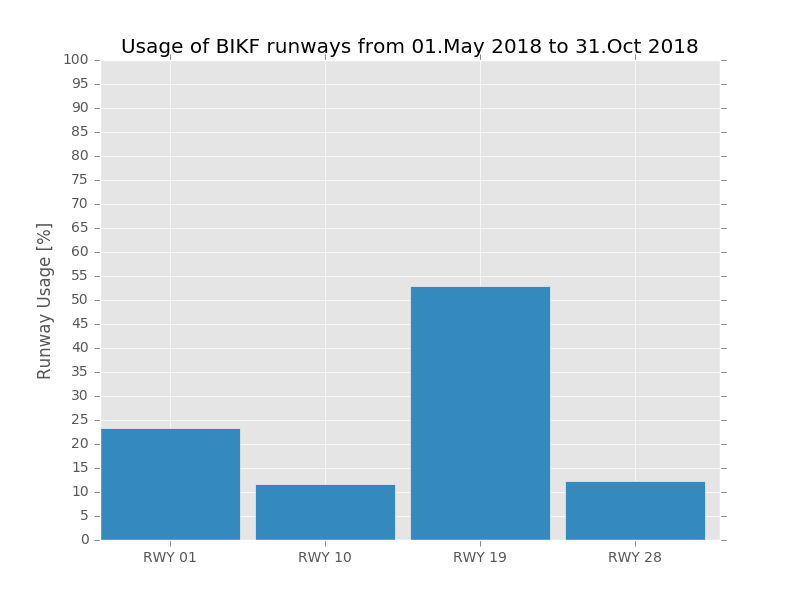
\includegraphics[width=0.7\textwidth]{graphics/fig_runway_usage_summer}
    \caption[Summer runway usage at BIKF]{The summer traffic favours RWY-19 (52,8\%), followed by RWY-01 (23,3\%), while RWY-10 and RWY-28 are with 11,6\% and 12,3\% respectively.}
    \label{fig:runway_usage_summer}
\end{figure}

\begin{figure}[h]
    \centering
    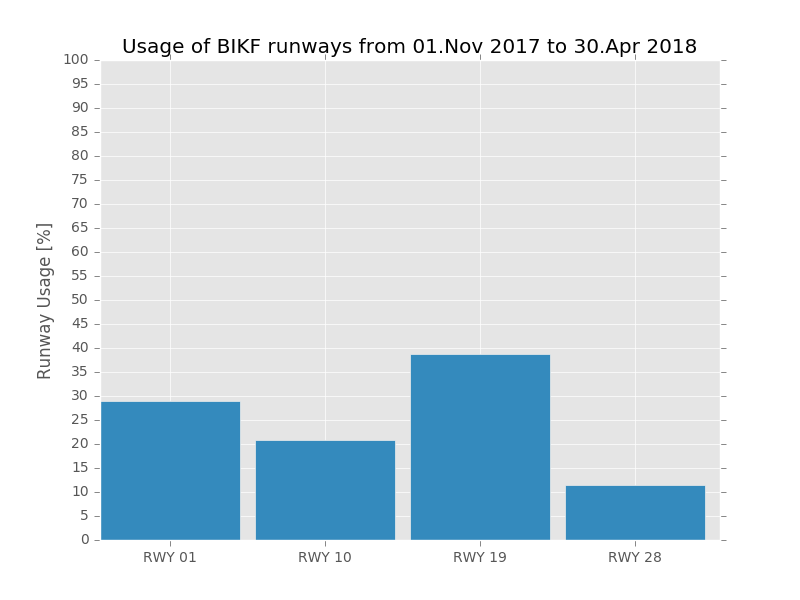
\includegraphics[width=0.7\textwidth]{graphics/fig_runway_usage_winter}
    \caption[Winter runway usage at BIKF]{The winter traffic at BIKF is slightly more evenly distributed among runways but still favours RWY-19 (38,8\%),followed by RWY-01 with 28,9\%, RWY-10 (20,8\%) and RWY-28 (11,4\%).}
    \label{fig:runway_usage_winter}
\end{figure}

\clearpage
\chapter{Arrival Runway Occupancy Times\label{app:AROTs}}





% Please add the following required packages to your document preamble:
% \usepackage{graphicx}
\begin{table}[h]
\centering
\resizebox{0.8\textwidth}{!} & \multicolumn{1}{l|}{50\%} & \multicolumn{1}{l|}{75\%} & \multicolumn{1}{l|}{max} \\ \hline
\multicolumn{1}{|l|}{RWY 01} & 963 & 85 & 21 & 46 & 68 & 88 & 100 & 152 \\ \hline
\multicolumn{1}{|l|}{RWY 10} & 852 & 85 & 11 & 61 & 78 & 84 & 91 & 155 \\ \hline
\multicolumn{1}{|l|}{RWY 19} & 1511 & 67 & 10 & 46 & 61 & 66 & 71 & 155 \\ \hline
\multicolumn{1}{|l|}{RWY 28} & 401 & 68 & 14 & 49 & 60 & 66 & 72 & 155 \\ \hline
\end{tabular}%
}
\caption[AROTs for the air traffic mix by runway for the summer]{AROT statistics for the air traffic mix at KEF by runway for the summer of 2018. The count is the number of landings during peak hours.}
\label{my-label3}
\end{table}

% Please add the following required packages to your document preamble:
% \usepackage{graphicx}
\begin{table}[h]
\centering
\resizebox{0.8\textwidth}{!} & \multicolumn{1}{l|}{50\%} & \multicolumn{1}{l|}{75\%} & \multicolumn{1}{l|}{max} \\ \hline
\multicolumn{1}{|l|}{RWY 01} & 290 & 88 & 26 & 47 & 63 & 90 & 106 & 153 \\ \hline
\multicolumn{1}{|l|}{RWY 10} & 338 & 93 & 12 & 70 & 85 & 91 & 100 & 144 \\ \hline
\multicolumn{1}{|l|}{RWY 19} & 259 & 72 & 13 & 51 & 65 & 69 & 75 & 140 \\ \hline
\multicolumn{1}{|l|}{RWY 28} & 69 & 73 & 13 & 49 & 63 & 72 & 79 & 105 \\ \hline
\end{tabular}%
}
\caption[AROTs for the air traffic mix by runway for the winter]{AROT statistics for the air traffic mix at KEF by runway for the winter season. The count is the number of landings during peak hours since October 2017}
\label{my-label4}
\end{table}

% Please add the following required packages to your document preamble:
% \usepackage{graphicx}
% \usepackage[table,xcdraw]{xcolor}
% If you use beamer only pass "xcolor=table" option, i.e. \documentclass[xcolor=table]{beamer}
\begin{table}[h]
\centering
\resizebox{0.8\textwidth}{!} & \multicolumn{1}{l|}{50\%} & \multicolumn{1}{l|}{75\%} & \multicolumn{1}{l|}{max} \\ \hline
\rowcolor[HTML]{DAE8FC} 
\multicolumn{1}{|l|}{\cellcolor[HTML]{DAE8FC}January} & 95 & 86 & 20 & 54 & 70 & 85 & 96 & 136 \\ \hline
\rowcolor[HTML]{DAE8FC} 
\multicolumn{1}{|l|}{\cellcolor[HTML]{DAE8FC}February} & 80 & 87 & 16 & 52 & 75 & 86 & 93 & 144 \\ \hline
\rowcolor[HTML]{DAE8FC} 
\multicolumn{1}{|l|}{\cellcolor[HTML]{DAE8FC}March} & 215 & 84 & 18 & 47 & 70 & 85 & 95 & 150 \\ \hline
\rowcolor[HTML]{DAE8FC} 
\multicolumn{1}{|l|}{\cellcolor[HTML]{DAE8FC}April} & 221 & 82 & 17 & 47 & 69 & 81 & 93 & 139 \\ \hline
\rowcolor[HTML]{FFFC9E} 
\multicolumn{1}{|l|}{\cellcolor[HTML]{FFFC9E}May} & 386 & 75 & 13 & 46 & 67 & 74 & 83 & 140 \\ \hline
\rowcolor[HTML]{FFFC9E} 
\multicolumn{1}{|l|}{\cellcolor[HTML]{FFFC9E}June} & 647 & 73 & 16 & 47 & 62 & 68 & 80 & 155 \\ \hline
\rowcolor[HTML]{FFFC9E} 
\multicolumn{1}{|l|}{\cellcolor[HTML]{FFFC9E}July} & 729 & 72 & 16 & 46 & 61 & 68 & 77 & 155 \\ \hline
\rowcolor[HTML]{FFFC9E} 
\multicolumn{1}{|l|}{\cellcolor[HTML]{FFFC9E}August} & 724 & 80 & 18 & 46 & 64 & 81 & 91 & 148 \\ \hline
\rowcolor[HTML]{FFFC9E} 
\multicolumn{1}{|l|}{\cellcolor[HTML]{FFFC9E}September} & 632 & 78 & 18 & 46 & 64 & 75 & 88 & 152 \\ \hline
\rowcolor[HTML]{FFFC9E} 
\multicolumn{1}{|l|}{\cellcolor[HTML]{FFFC9E}October} & 609 & 79 & 17 & 46 & 66 & 76 & 91 & 155 \\ \hline
\rowcolor[HTML]{DAE8FC} 
\multicolumn{1}{|l|}{\cellcolor[HTML]{DAE8FC}November} & 239 & 84 & 23 & 48 & 66 & 82 & 99 & 151 \\ \hline
\rowcolor[HTML]{DAE8FC} 
\multicolumn{1}{|l|}{\cellcolor[HTML]{DAE8FC}December} & 106 & 87 & 23 & 51 & 69 & 86 & 99 & 153 \\ \hline
\end{tabular}%
}
\caption[AROTs for the air traffic mix by month]{AROT statistics for the air traffic mix at BIKF by month. The count is the number of landings during peak hours from October 2017 til November 2018. The colour fields indicate a subjective separation of the data into summer and winter season, based on mean AROT value. Months with mean AROT $\leq$ 80 seconds were classified as summer, and the remaining as winter.}
\label{tab:month2season_arot}
\end{table}

\clearpage
\chapter{Landing time interval and AROT}\label{app:lti_and_arot}

% \begin{figure}[h]
%     \centering
%     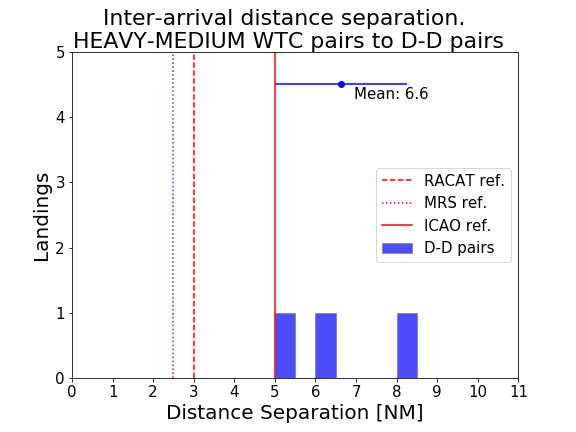
\includegraphics[width=0.5\textwidth]{graphics/fig_HM_to_DD_pairs_dist_separ.png}
%     \caption[Inter-arrival distance separation of H-M pairs to D-D pairs into the RECAT-EU scheme]{Inter-arrival distance separation after re-categorisation of H-H pairs to D-D pairs into the RECAT-EU scheme.}
%     \label{fig:HM_to_DD_pairs_dist_separ}
% \end{figure}


% Please add the following required packages to your document preamble:
% \usepackage{multirow}
% \usepackage{graphicx}
\begin{table}[h]
\centering
\resizebox{0.8\textwidth}{!}{%
\begin{tabular}{|c|c|c|c|c|c|c|c|}
\hline
\multicolumn{2}{|c|}{\multirow{2}{*}{RECAT-EU scheme}} & \multicolumn{6}{c|}{Follower}                   \\ \cline{3-8} 
\multicolumn{2}{|c|}{}& CAT-A & CAT-B & CAT-C & CAT-D & CAT-E & CAT-F \\ \hline
\multirow{6}{*}{\rotatebox[origin=c]{90}{Leader}}& CAT-A&& 100s  & 120s  & 140s  & 160s  & 180s  \\ \cline{2-8}
& CAT-B&&&& 100s  & 120s  & 140s  \\ \cline{2-8} 
& CAT-C&&&& 80s   & 100s  & 120s  \\ \cline{2-8} 
& CAT-D&&&&&& 120s  \\ \cline{2-8} 
& CAT-E&&&&&& 100s  \\ \cline{2-8} 
& CAT-F&&&&&& 80s   \\ \hline
\end{tabular}%
}
\caption[RECAT-EU time-based separation minima]{RECAT-EU WT time-based separation minima on approach and departure~\cite{rooseleer2015recat}}
\label{tab:RECAT-time}
\end{table}





\clearpage
\chapter{ADS-B Standard Data Items}\label{app:adsb_items}

\begin{figure}[h]
    \centering
    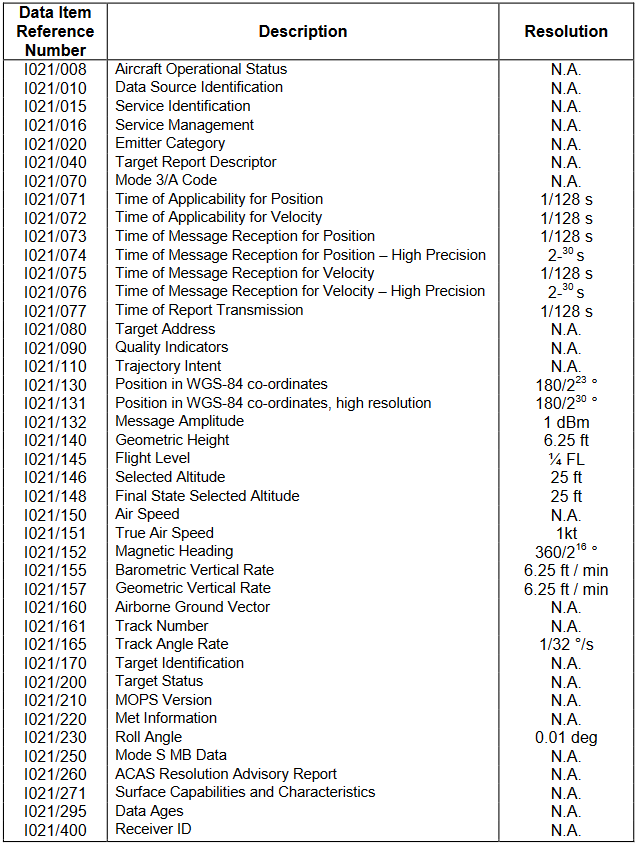
\includegraphics[width=0.7\textwidth]{graphics/ads_b_items.png}
    \caption[ADS-B Standard Data Items]{ADS-B Standard Data Items \cite[p. 8]{ASTERIX_ADS-B_specs}.}
    \label{fig:adsb_items}
\end{figure}


\clearpage
\chapter{BIKF Wind Rose}\label{app:wind_rose}

\begin{figure}[h]
    \centering
    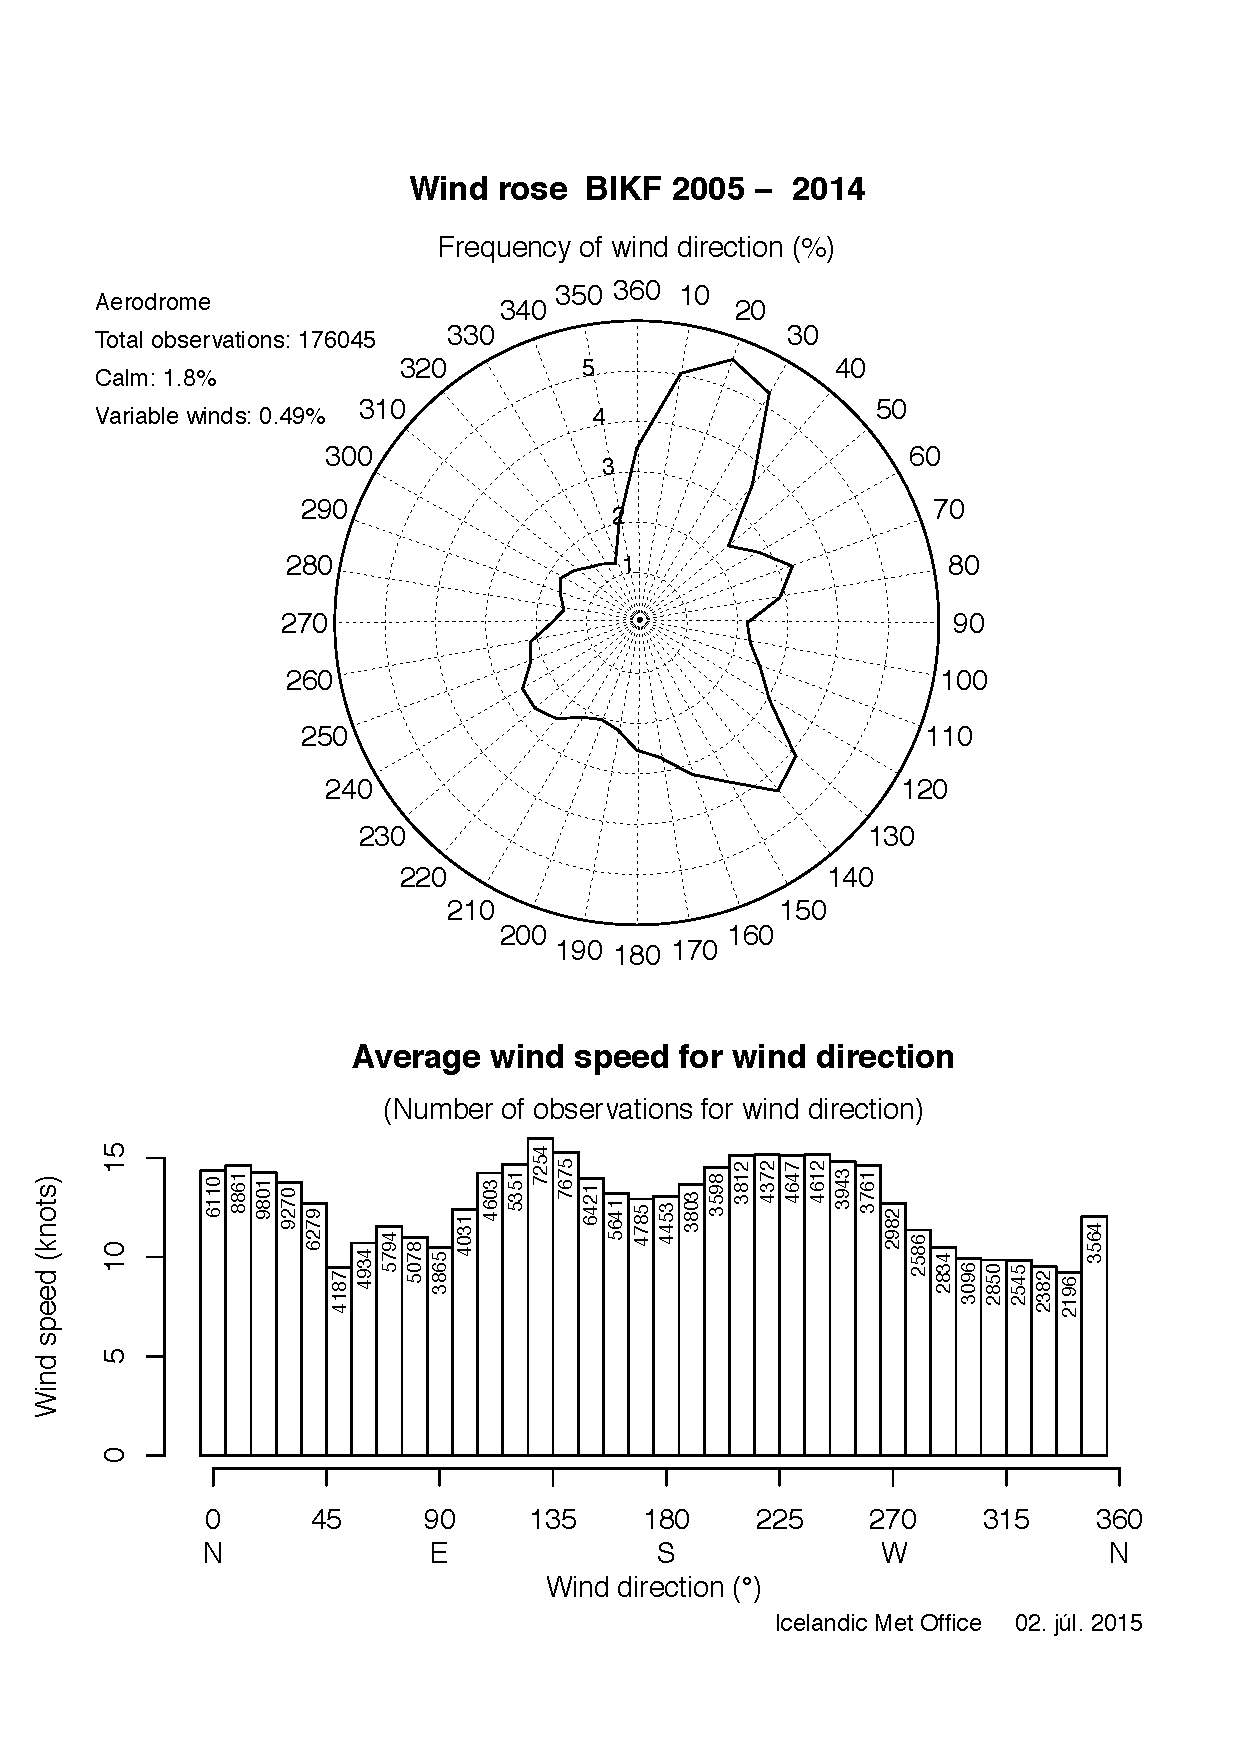
\includegraphics[width=0.7\textwidth]{graphics/BIKF_windrose_2005-2014.pdf}
    \caption[BIKF Wind Rose]{Wind rose - frequency, direction and strength of winds at BIKF aerodrome \cite{wind_rose_2014}.}
    \label{fig:BIKF_wind_rose}
\end{figure}
% ----------------------------


% \chapter{Code}\label{cha:code}
% You can put code in your document using the listings package, which is
% loaded by default in \path{custom.tex}.  Be aware that the listings
% package does not put code in your document if you are in draft mode
% unless you set the \texttt{forcegraphics} option.

% There is an example java (Listing~\ref{src:Data_Bus.java}) and XML
% file (Listing~\ref{src:AndroidManifest.xml}).  Thanks to the
% \texttt{url} package, you can typeset OSX and unix paths like this:
% \path{/afs/rnd.ru.is/project/thesis-template}.  Windows paths:
% \path{C:\windows\temp\ }.  You can also typeset them using the menukey
% package, but it tends to delete the last separator and has other
% complications.\footnote{The menukey package has issues with biblatex,
%   read \path{custom.tex} for more information.}

% If you are trying to include multiple different languages, you should
% go read the documentation and set these up in \path{custom.tex}.  You
% will save yourself a lot of effort, especially if you have to fix
% anything.

% %I have put the source code in the \directory{src/} folder.
% \lstinputlisting[language=Java, firstline=1,
% lastline=40, caption={Data\_Bus.java: Setting up the class.},
% label={src:Data_Bus.java}]{src/Data_Bus.java}

% \lstinputlisting[language={[android]XML}, firstline=1, lastline=20,
% caption={AndroidManifest.xml: Configuration for the Android UI.},
% label={src:AndroidManifest.xml}]{src/AndroidManifest.xml}

%%% Local Variables: 
%%% mode: latex
%%% TeX-master: "DEGREE-NAME-YEAR"
%%% End: 
